%!TEX TS-program = xelatex
%!TEX root = ../../maxwell2018thesis.tex

\chapter[The Complex Searcher Model]{The Complex Searcher Model}\label{chap:csm}
In this chapter, we present the~\gls{acr:csm}, an updated searcher model that is one of the major contributions of this thesis. The~\gls{acr:csm} is an amalgamation and further development of prior, established searcher models that capture the interactions taking place between a searcher and a retrieval system.

As discussed in Section~\ref{sec:ir_background:user:models}, prime examples of prior searcher models include the Markov-based approach presented by~\cite{baskaya2013behavioural_factors}, and the model proposed by~\cite{thomas2014modelling_behaviour}. These searcher models (along with others) are in broad agreement with the general sequence of events that take place within the~\gls{acr:iir} process -- from issuing a query, to examining documents for relevance.



\begin{figure}[t!]
    \centering
    \resizebox{1\hsize}{!}{
    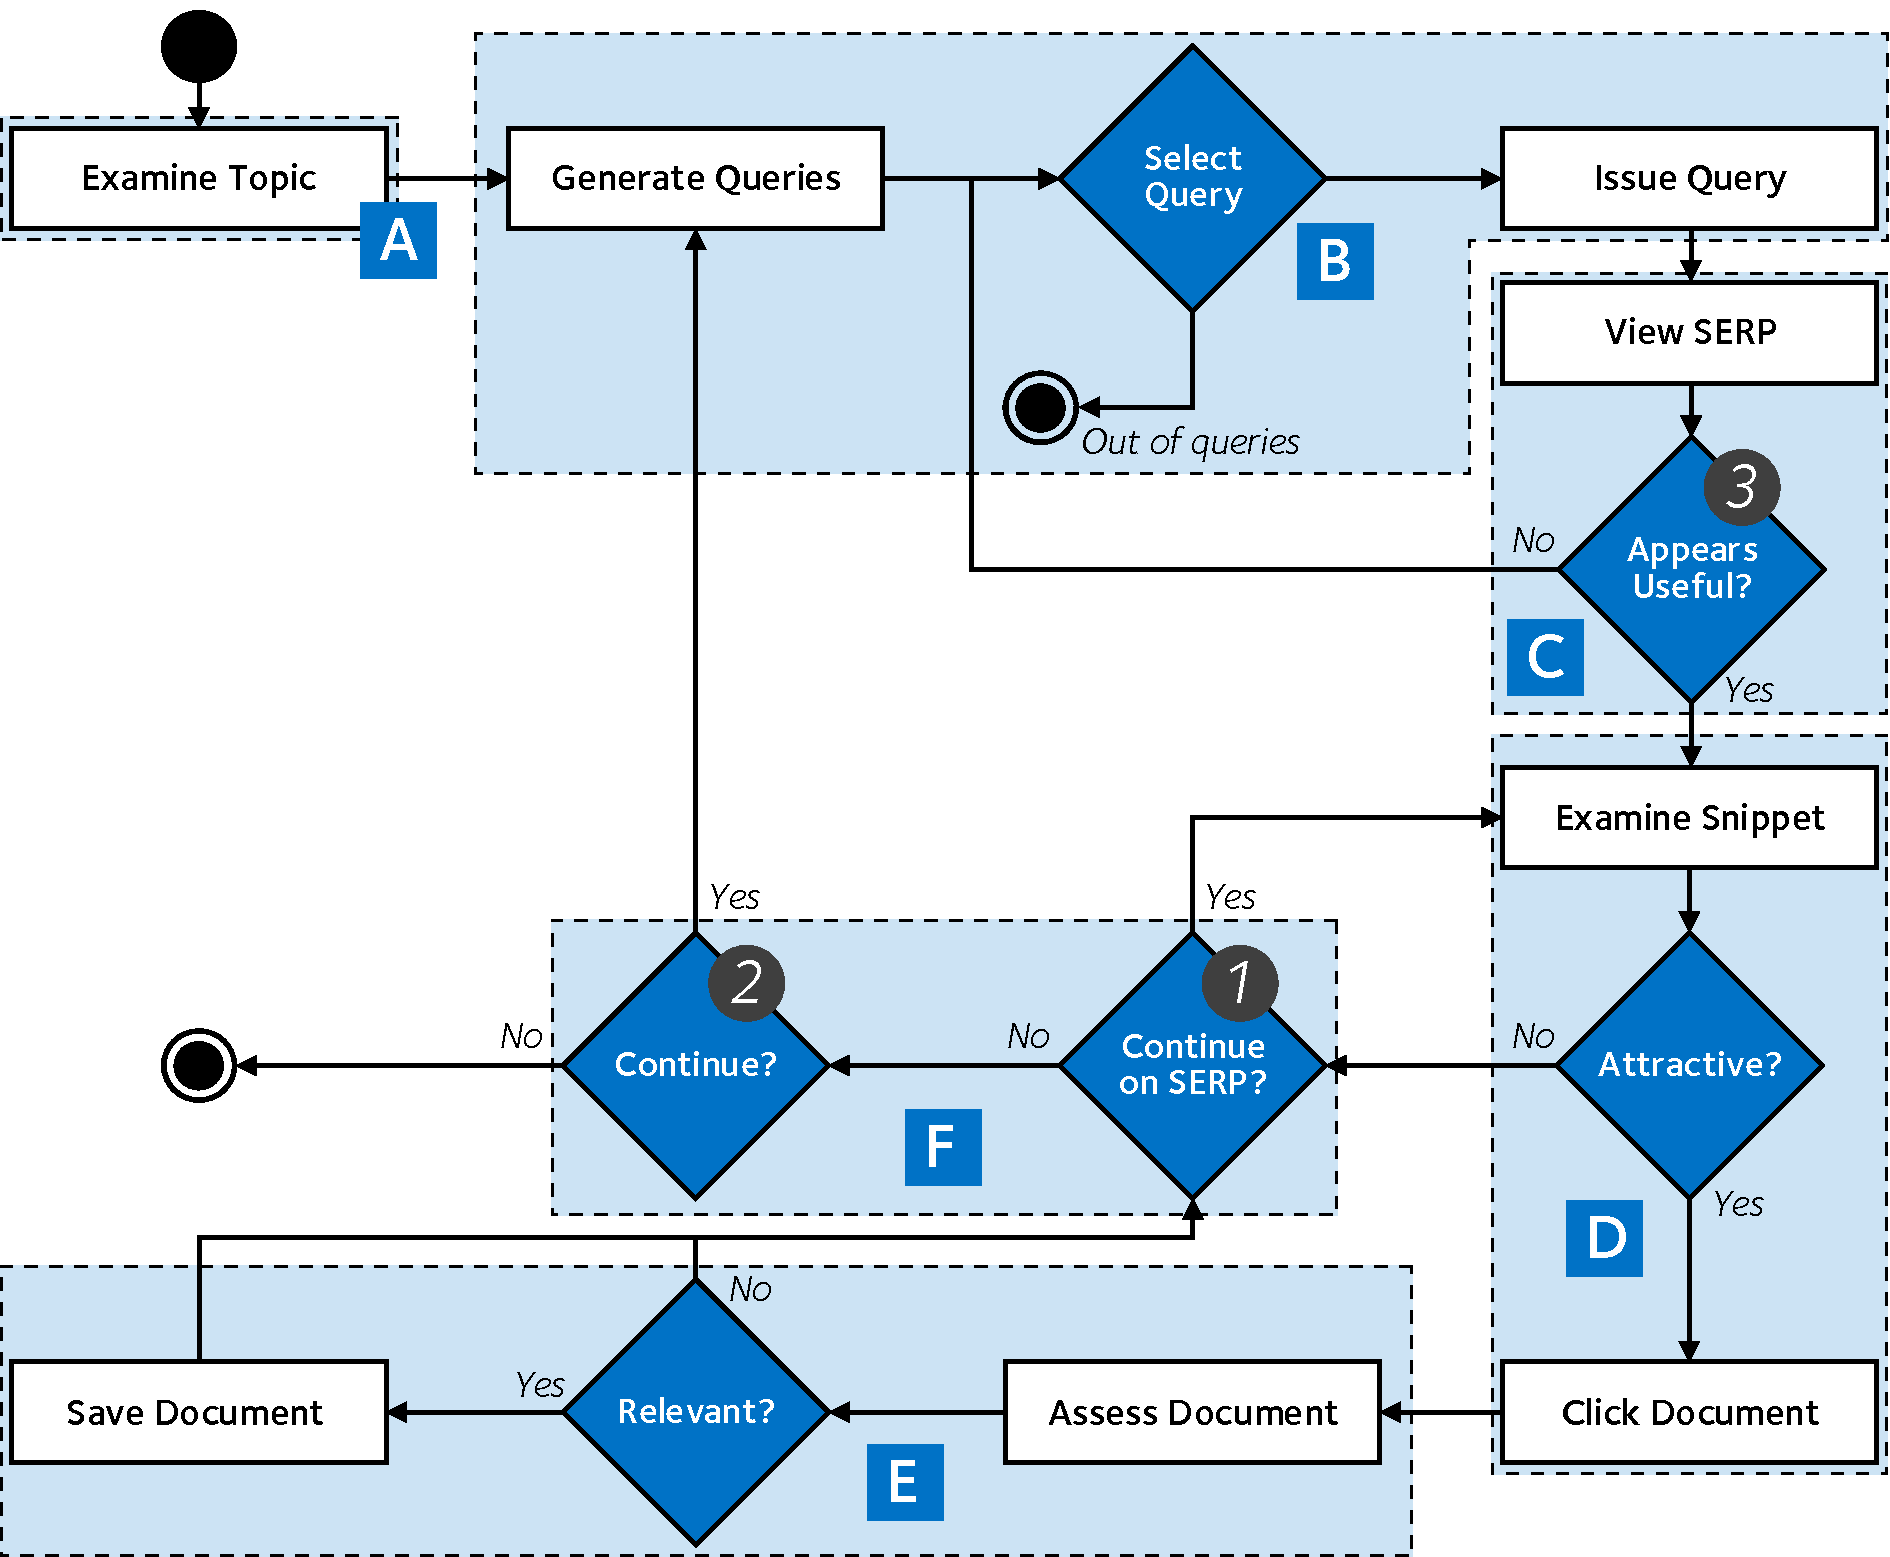
\includegraphics{figures/ch4-csm.pdf}}
    \caption[Flowchart of the~\glsfirst{acr:csm}]{A flowchart of the proposed~\glsfirst{acr:csm}, as used in experimental work discussed later in this thesis. Novel components that the work this thesis provides are highlighted by boxes \blueboxbold{A} and \blueboxbold{B}. The \emph{three} stopping decision points are highlighted with \blueboxbold{1}, \blueboxbold{2} and \blueboxbold{3} (refer to Section~\ref{sec:csm:stopping}). Refer to Section~\ref{sec:csm:csm:flow} for an in-depth explanation of the model.}
    \label{fig:csm}
\end{figure}